\newpage

\section{PseudoCylindrical projections}
\subsection{Robinson}
\begin{figure}[H]
    \centering
    \begin{minipage}{0.30\textwidth}
        \centering
        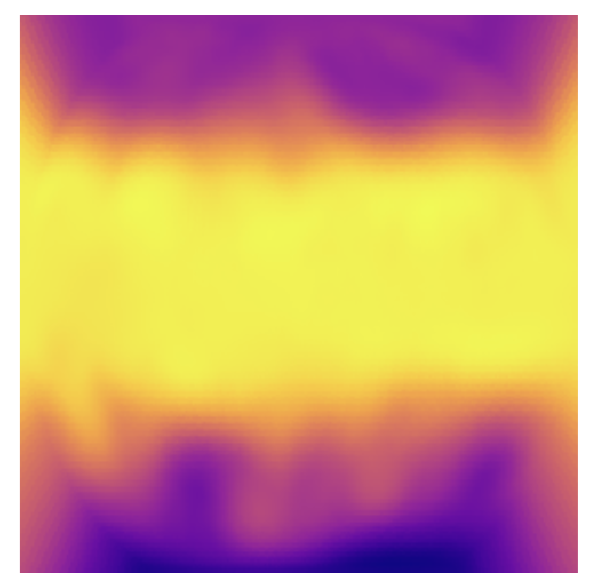
\includegraphics[width=0.9\linewidth]{figures/chapter-8/geopoth_robin.png}
        \caption{ Geopotential height raster data as Robinson projected}
        \label{fig:robin_geopoth_raster}
    \end{minipage}\hfill
    \begin{minipage}{0.30\textwidth}
        \centering
        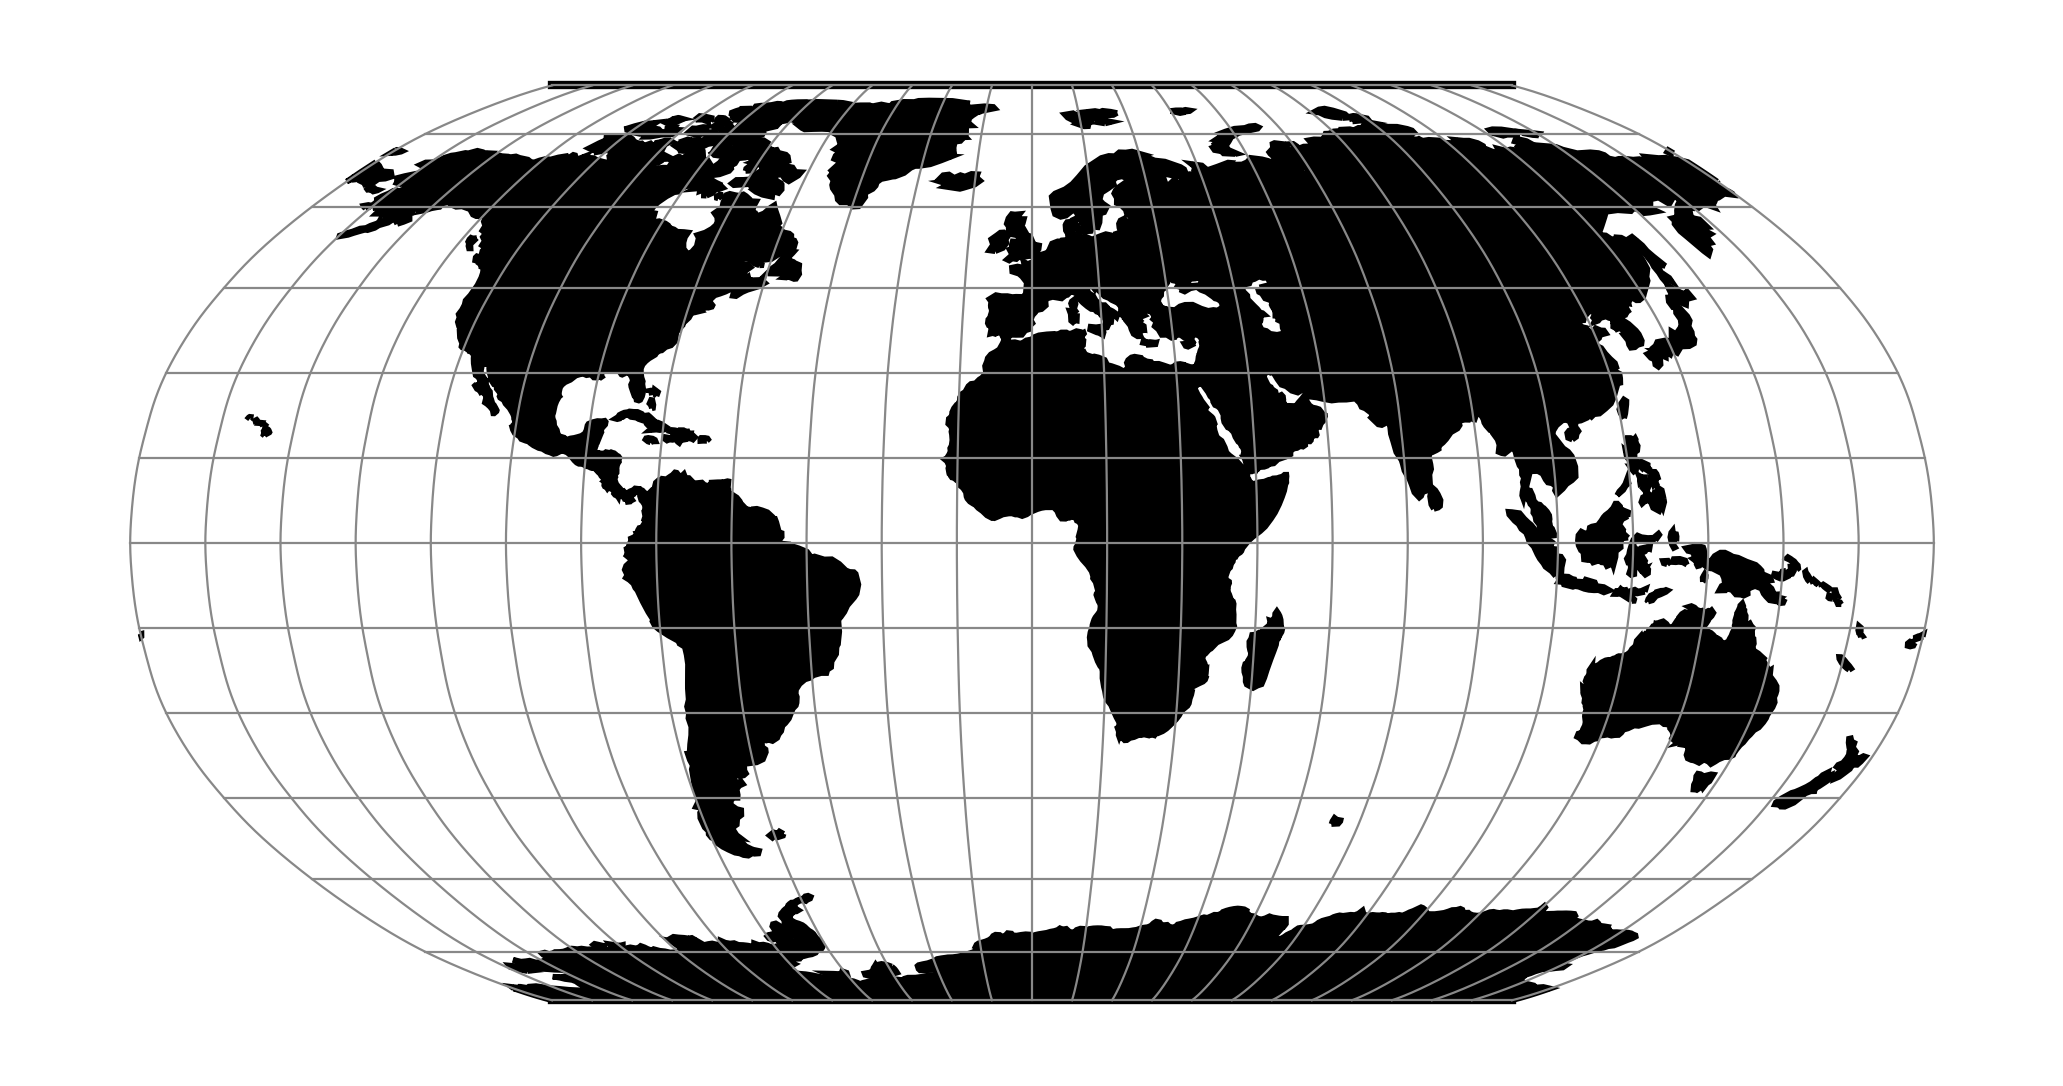
\includegraphics[width=0.9\linewidth]{figures/chapter-8/robin.png}
        \caption{Robinson (Source \cite{PROJ_SITE})}
        \label{fig:robin_proj}
    \end{minipage}\hfill
    \begin{minipage}{0.30\textwidth}
        \centering
        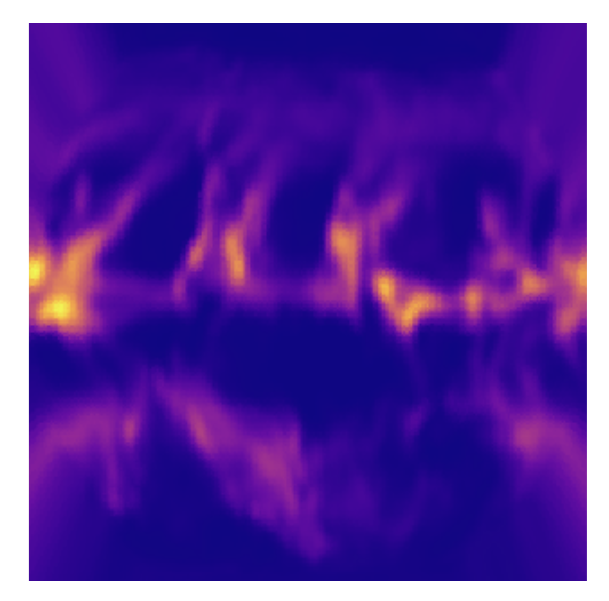
\includegraphics[width=0.9\linewidth]{figures/chapter-8/prect_robin.png}
        \caption{Precipitation raster data as Robinson projected}
        \label{fig:robin_prect_raster}
    \end{minipage}\hfill
\end{figure}
\begin{figure}[H]
    \centering
    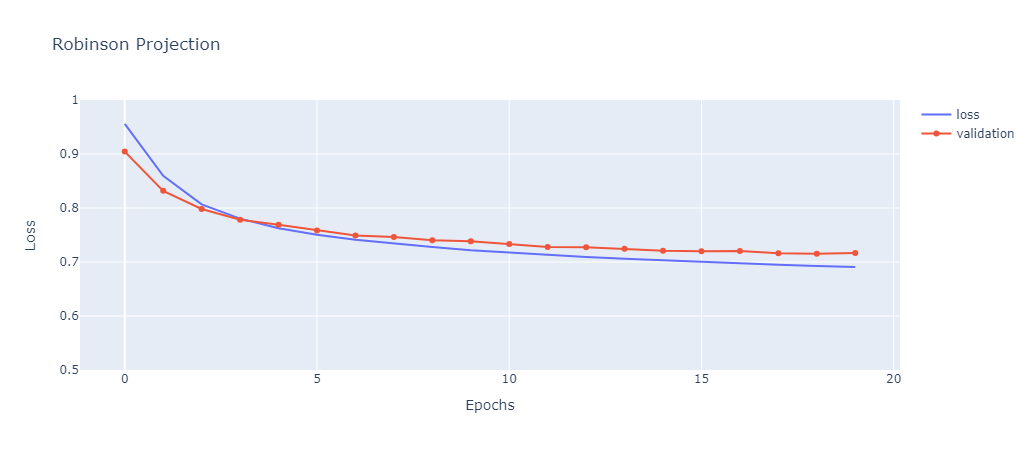
\includegraphics[width=1.0\linewidth]{figures/chapter-8/robin_loss.png}
    \caption{Robinson: Averaged training loss of models  }
    \label{fig:robin_loss}
\end{figure}
\subsection{Interrupted Goode Homolosine}
\begin{figure}[h]
    \centering
    \begin{minipage}{0.30\textwidth}
        \centering
        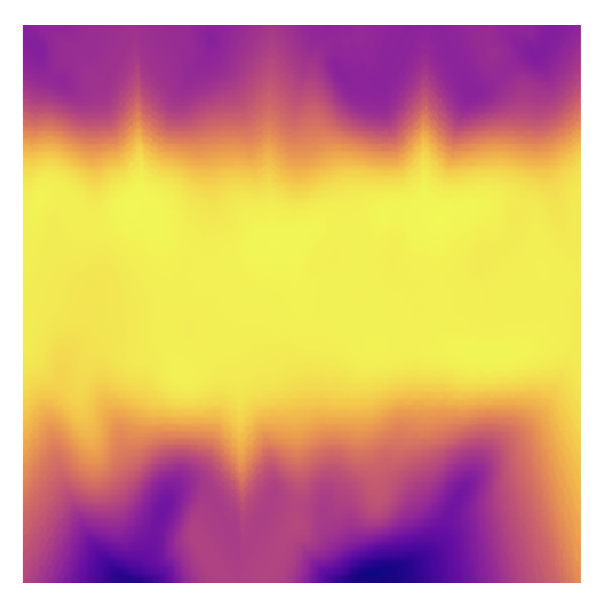
\includegraphics[width=0.9\linewidth]{figures/chapter-8/geopoth_goode.png}
        \caption{ Geopotential height raster data as Interrupted Goode Homolosine projected}
        \label{fig:ig_geopoth_raster}
    \end{minipage}\hfill
    \begin{minipage}{0.30\textwidth}
        \centering
        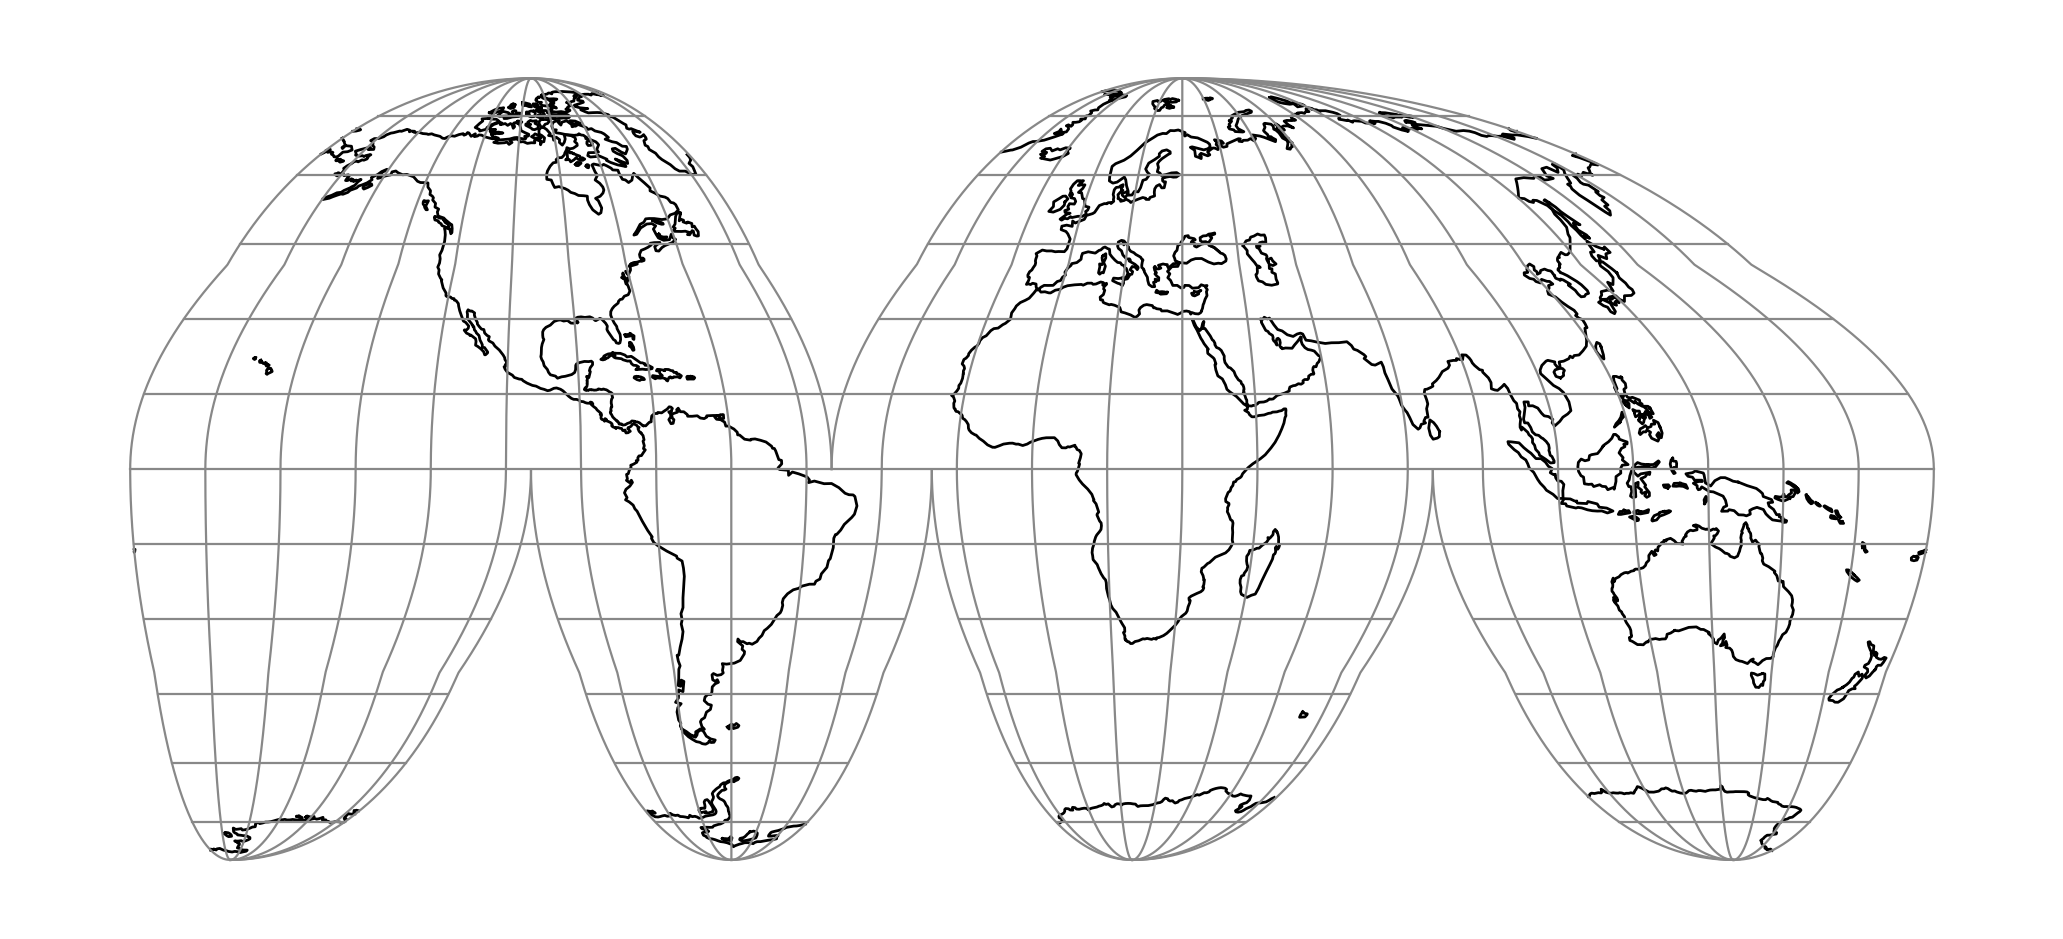
\includegraphics[width=0.9\linewidth]{figures/chapter-8/igh.png}
        \caption{Interrupted Goode Homolosine (Source \cite{PROJ_SITE})}
        \label{fig:ig_proj}
    \end{minipage}\hfill
    \begin{minipage}{0.30\textwidth}
        \centering
        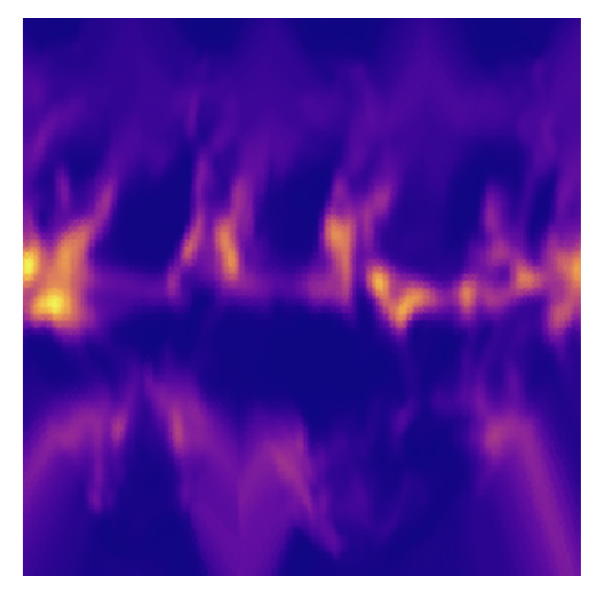
\includegraphics[width=0.9\linewidth]{figures/chapter-8/prect_goode.png}
        \caption{Precipitation raster data as Interrupted Goode Homolosine projected}
        \label{fig:ig_prect_raster}
    \end{minipage}\hfill
\end{figure}

\begin{figure}[H]
    \centering
    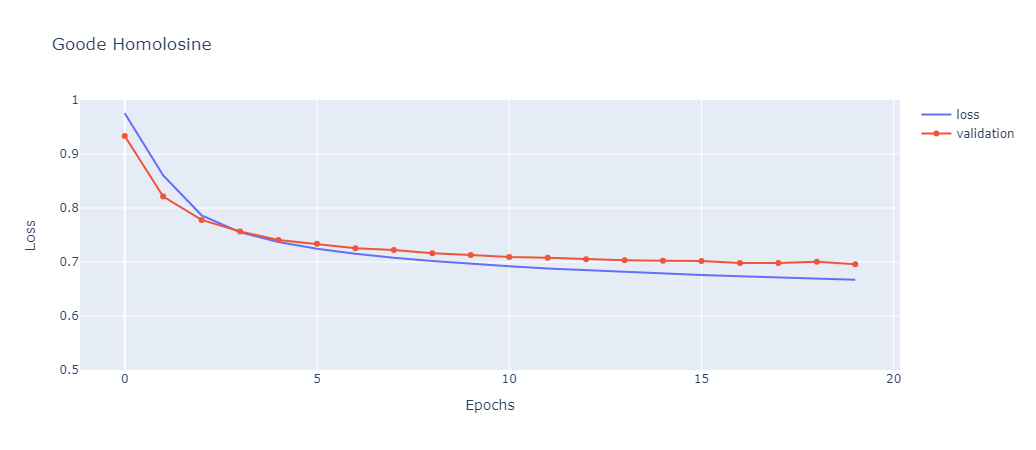
\includegraphics[width=1.0\linewidth]{figures/chapter-8/goode_loss.png}
    \caption{Interrupted Goode Homolosine: Averaged training loss of models  }
    \label{fig:goode_loss}
\end{figure}
\subsection{Sinusoidal Sanson Flamsteed}
\begin{figure}[H]
    \centering
    \begin{minipage}{0.30\textwidth}
        \centering
        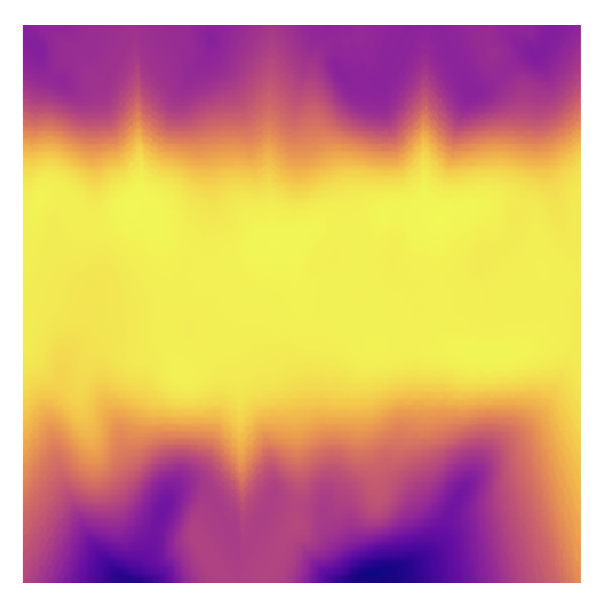
\includegraphics[width=0.9\linewidth]{figures/chapter-8/geopoth_goode.png}
        \caption{ Geopotential height raster data as Sinusoidal Sanson Flamsteed projected}
        \label{fig:ig_geopoth_raster}
    \end{minipage}\hfill
    \begin{minipage}{0.30\textwidth}
        \centering
        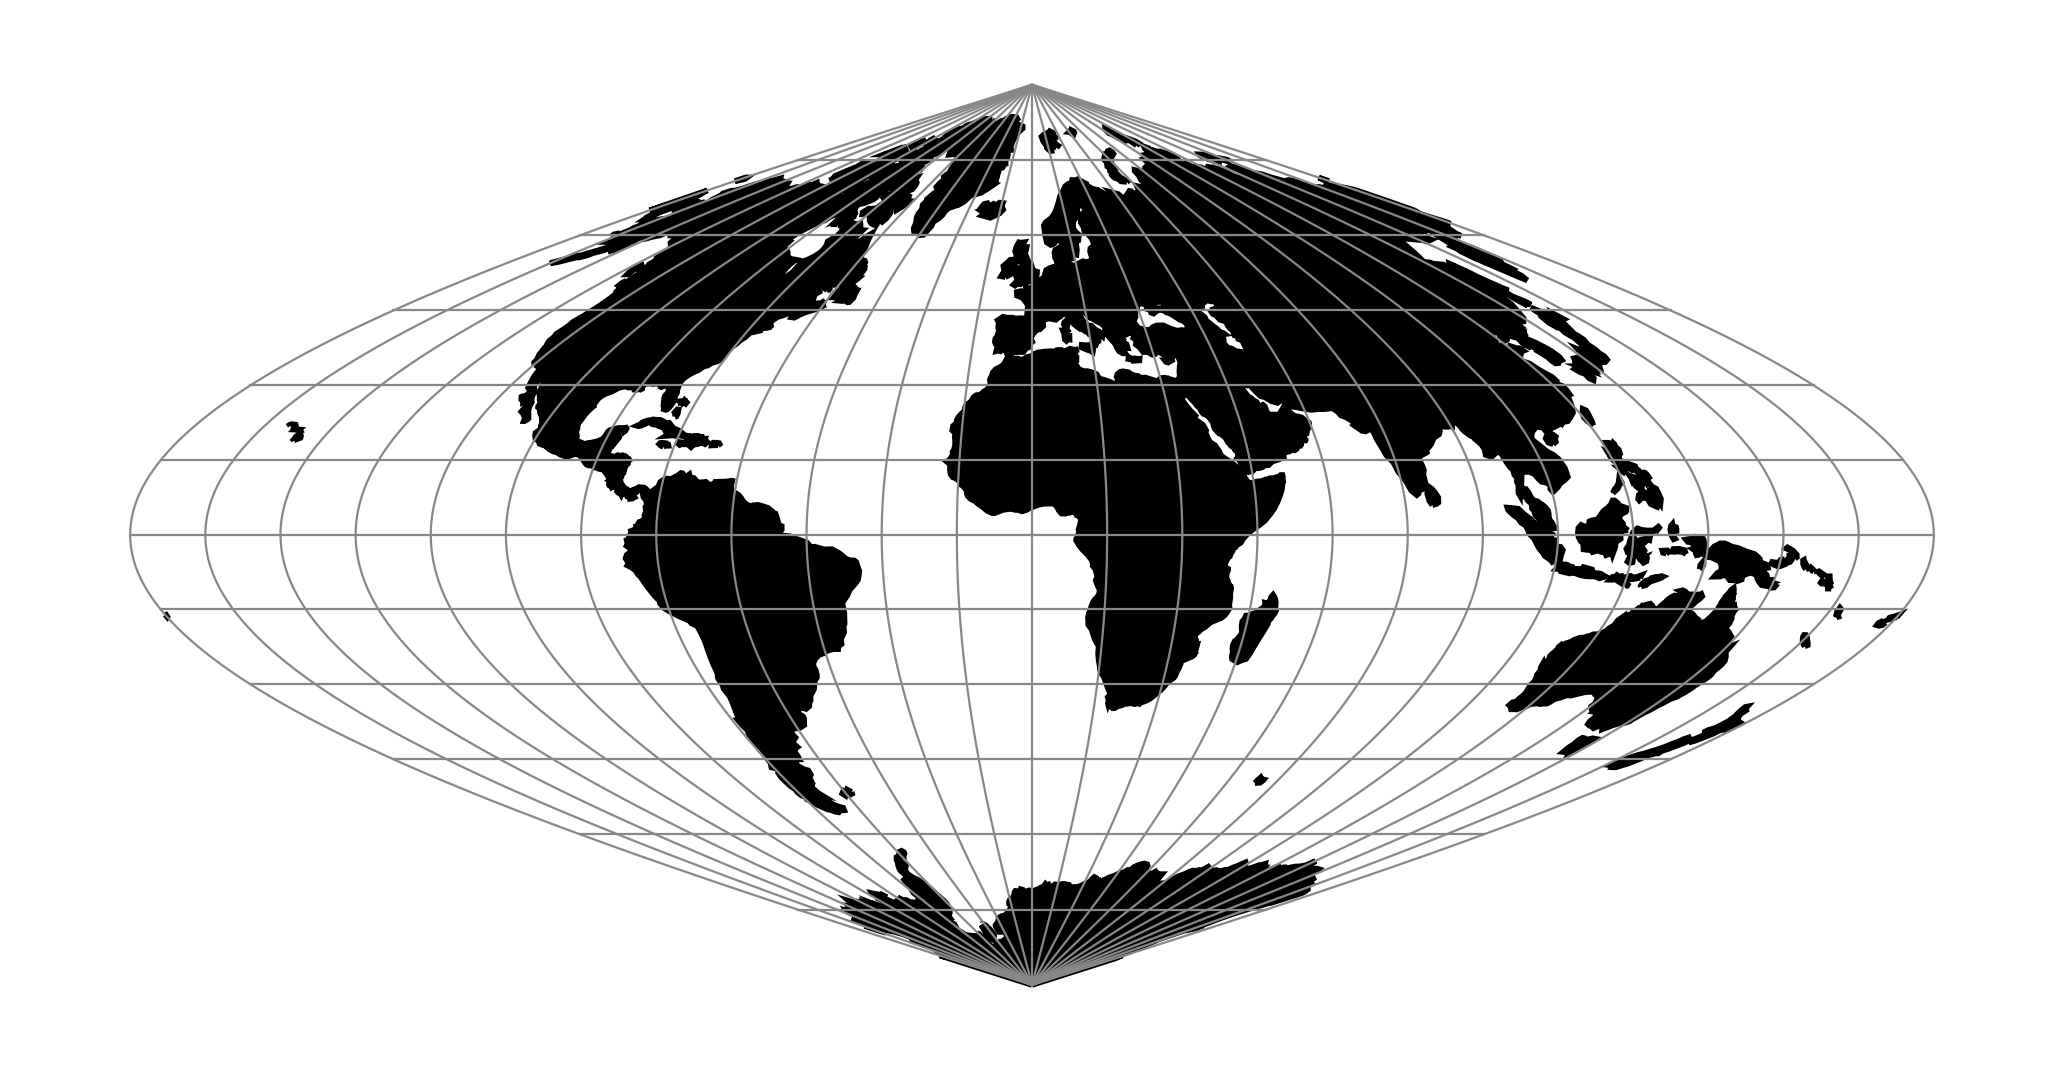
\includegraphics[width=0.9\linewidth]{figures/chapter-8/sinu.png}
        \caption{Sinusoidal Sanson Flamsteed (Source \cite{PROJ_SITE})}
        \label{fig:ig_proj}
    \end{minipage}\hfill
    \begin{minipage}{0.30\textwidth}
        \centering
        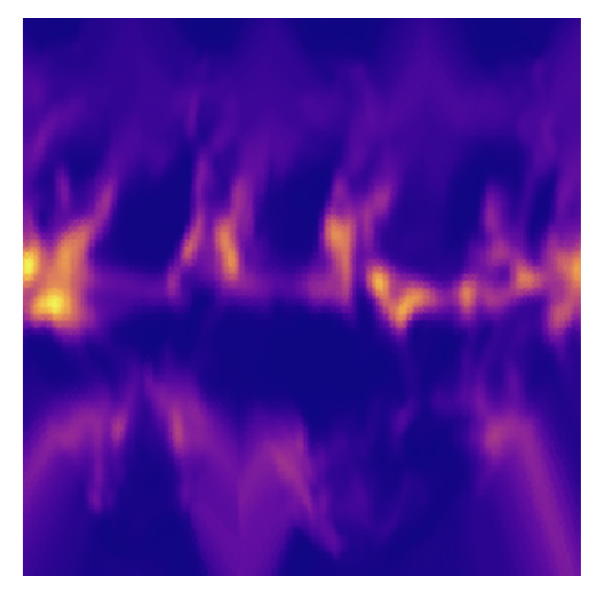
\includegraphics[width=0.9\linewidth]{figures/chapter-8/prect_goode.png}
        \caption{Precipitation raster data as Sinusoidal Sanson Flamsteed projected}
        \label{fig:ig_prect_raster}
    \end{minipage}\hfill
\end{figure}


\begin{figure}[H]
    \centering
    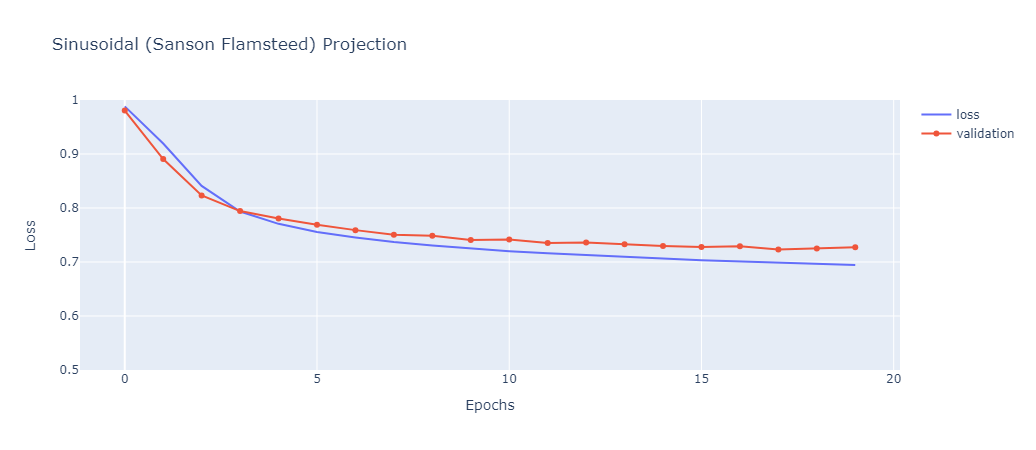
\includegraphics[width=1.0\linewidth]{figures/chapter-8/sinu_loss.png}
    \caption{Sinusoidal Sanson Flamsteed: Averaged training loss of models  }
    \label{fig:sinu_loss}
\end{figure}

\subsection{Loximuthal}
\subsection{Results}
\begin{table}[ht]
    \centering
    \caption{Summary of Model Performance}
    \label{pseudo_cylindrical_results_table}
    \renewcommand{\arraystretch}{1.2} % Adjusts the row height
    \begin{tabular}{|l|c|c|c|c|c|}
        \hline
        \rowcolor[gray]{0.9}
        \textbf{\emph{Project Name}} & \textbf{\emph{\# Epochs}} & \textbf{\emph{MAE}} & \textbf{\emph{Validation MAE}} & \textbf{\emph{MAPE}} & \textbf{\emph{Validation MAPE}} \\ \hline
        Project 1                    & 50                        & 0.05                & 0.06                           & 5\%                  & 6\%                             \\ \hline
        Project 2                    & 30                        & 0.04                & 0.05                           & 4\%                  & 5\%                             \\ \hline
        Project 3                    & 100                       & 0.03                & 0.04                           & 3\%                  & 4\%                             \\ \hline
    \end{tabular}
\end{table}
